\chapter{From Theory To Practice}
\label{implementation}

This section describes all the optimizations , implementation decisions and details of Narukom. The primary goal of Narukom is to be used as a communication
framework in robotic environments, so most of our choices were in favour of real-time embedding systems and specifically for the Standard Platform League
competition. Consequently, Narukom does not fit in all problem domains.
\section{Understanding the basics}
\subsection{Messages}
The exchanged data between the threads are protocol buffers messages, defined by the user. Narukom requires to include in each message definition some attributes that are of outmost importance in order for Narukom to work properly and handle every message. As metioned before, every message definition in Narukom takes the following form with five mandatory attributes in its preamble: 
\begin{verbatim}
message xxxMessage{
    required string host      = 1 [default = "localhost"];
    required string publisher = 2 [default = "" ];
    required string topic     = 3 [default = "global"];
    required int32  timeout   = 4 [default = 0];
    required string  timestamp = 5 [default = ""];
    < attributes specific to the xxxMessage type >
}
\end{verbatim} 
Narukom includes a definition of a basic structure called BasicMessage in order to deal with all the messages. Each attribute serves a purpose,
\begin{itemize}
\item {\tt host,publisher} attributes are used in order to distinguish messages from the between network nodes,
\item {\tt topic} is the topic in which each message should be published and
\item {\tt timeout,timestamp} are the temporal information needed by \textit{Narukom} for synchronization purposes.
\end{itemize}

\subsection{MessageBuffer}
This structure is a thread safe and as its name suggests, is a buffer in which protocol buffer messages are stored. Apart from the simple vector to hold the messages, the structure has a string attribute named {\tt owner} ,which denotes the name of the owner of the buffer. It must be noted that message buffer is implemented as monitor.

\section{Publish/Subscribe system in \textit{Narukom} }
Publish/Subscribe implementation is shown in figure ~\ref{fig:Narukom-publish-subscribe}.



\begin{figure}[t]
\centering
  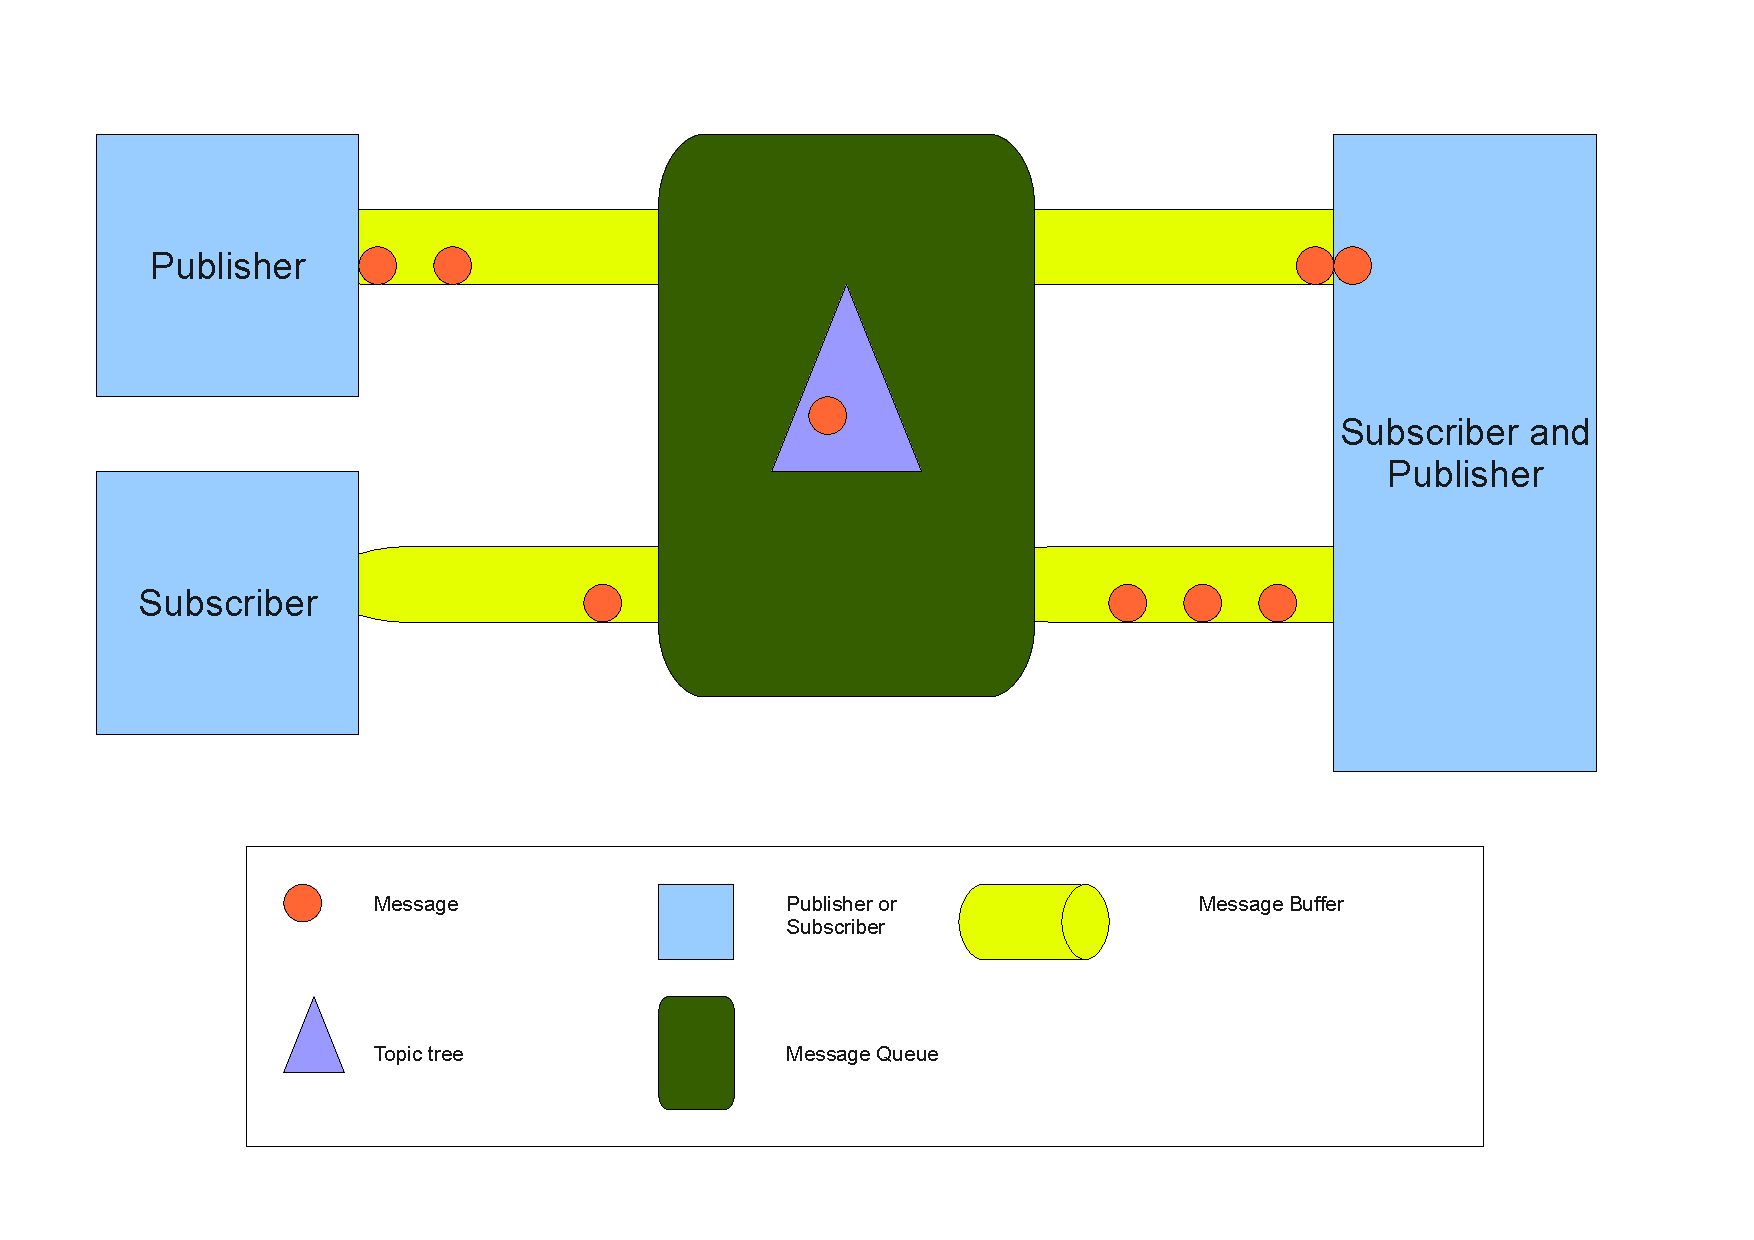
\includegraphics[width=0.9\columnwidth]{Chapter4/figures/publish_subscribe.pdf}
  \caption{Narukom's publish/subscribe implementation.} 
  \label{fig:Narukom-publish-subscribe}
\end{figure}
Both publishers and subscribers have one message buffer through which the exchange of data takes place. Message queue, periodically checks all the publishers'
buffers and copies them to the buffers of all interested subscribers. This approach minimizes the race conditions when accessing messages , on the cost of high
decoupling between the publishers and subscribers , which in real-time systems could be source of undesirable behavior. In the next section , it is described
how this problem is addressed. Continuing with the publish/subscribe system, in order for classes use the infrastructure provided by Narukom , should inherit
from either  {\tt Publisher } or {\tt Subscriber} class ( or both ). Although , there is a default implementation of the interfaces for both classes, it is
recommended  derived classes not to rely on the default implementation as it might have undesirable effects on the behavior of their system. The
 {\tt Publisher } class requires the implementation of the  method:
\begin{verbatim}
void publish( google::protobuf::Message* msg)
\end{verbatim}
The default implementation of this method just adds the \textit{msg} message to the buffer, which in the majority of the scenarios would be a sufficient
behavior for sending a message.
On the other hand , classes derived from {\tt Subscriber} class  is strongly encouraged to provide their own implementation of the  method: \footnote{The default implementation of the process\_messages() is provided just as a reference.}
\begin{verbatim}
void process_messages()
\end{verbatim}


\subsection{Message Queue}
Message queue performance affects directly the overall performance of our system, thus several optimizations have been made to this class. The most
important optimization is that the internal topic tree is used as a reference structure, while the actual data structure used is a hash table on all the  topics the tree included. The configuration of the tree is done via an XML file on each node, on the initialization of the message queue the file is parsed and the tree is created.
 The hash table gives us fast retrieval on the list of subscribers to which the arrived message must be delivered. Furthermore, when it comes to reading  the message's meta-data, a cast to  {\tt BasicMessage} type is used, overriding the normal way of accessing
data in protocol buffers. It must be stressed that this approach is used ONLY for reading and ONLY in \textbf{Blackboard and Message Queue} classes. \textbf{under no circumstances is recommended as the normal way for accessing the meta-data required by Narukom}. This is considered a heavy optimization which could stop working after a new release of protocol buffers.  Last but not least, instead of keeping pointers to the publisher or subscriber , a message buffer pointer is used in order to avoid the small overhead of calling an extra method every time {\tt Message Queue} needs to access a buffer. As insignificant as these optimizations may seem , in (SPL) ,where software makes the difference, they could decide the winner of a game.

\section{Blackboard and Synchronization}
The implemented publish/subscribe system maximizes the decoupling between publishers and subscribers, thus a lot synchronization issues might arise between
threads running locally on a node. this problem is dealt, by adding two attributes in the meta-data of each message . Narukom introduces some conventions for
each message, when a message is published a timestamp is assigned ( at least in the default implementation of publish ), at the time the subscriber receives a
message should check the validity of the data by ensuring that those data are not expired, on data expiration subscribers are advised to dispose those
messages in order to limit the excess and unusable information on a node. It should be noted that those are convention of Narukom that are used internally and
cannot be imposed on subscribers, each subscriber is free to comply or not with them. Narukom's blackboard utilizes the time information to minimize memory
allocation and provide synchronization services to the higher level system. Blackboard implementation creates two indexes over the stored messages, one to
provide fast access for data requests and another to provide fast cleanup time. The latter index is an ordered list in terms of absolute timeout calculated
when new messages are stored in the blackboard. Frequently, the blackboard cleans up all the expired data.


\section{Communication across nodes}
Communication between the nodes of Narukom is achieved through channels, which are  well-defined pairings between actuators (motors, speakers, network adapter) affecting the robot's environment, whereas  sensors (camera, microphones,network adapters) sense the robots environment. Narukom was designed in order to be able to utilize all the individual channels, to tackle with the wide range of features and integrate those channels in the framework catalog module introduced.

\section{Catalog Module}
Catalog module could be characterized as the address book of each node in Narukom , since it holds all the contact information of all the reachable peers by the node itself. Furthermore, Catalog is responsible for creating and destroying the various channels that the node is able to use in order to communicate with other nodes.  The idea behind this module is that in distributed environments a node must be aware of all the available nodes and what type of service they provide. In detail,  the information  stored in a catalog module are names of all reachable peers, through which channels are these nodes available and which kind of data are interested in. Moreover, catalog holds a list of all the usable channels on the node and has the ability to start, stop or filter the type of messages that are sent through each channel. The filtering is done by sending commands that a channel can interpret into one of the above functions. These commands are a protocol buffer message with the following attributes
\begin{verbatim}
message ChannelCommand{
required string type = 1 [default = ""];
required string element = 2 [ default = "none"];
}
\end{verbatim} 
There are four different types of commands
\begin{itemize}
\item{\tt subscribe}, when this type of message is received, a channel must subscribe on a certain topic.
\item{\tt unsubscribe}, a channel should unsubscribe from a topic
\item{\tt enable}, this command is used to enable a specific type of message to be sent through it, by default after the subscription of a channel all the incoming messages are enabled and the
\item{\tt disable}, obviously this is the opposite of the enable command.
\end{itemize}
The attribute element is in accordance with the command type , in case of (un)subscribe , it should hold the topic , whereas when sending an enable or disable command it must be a type of message. Channels should implement a simple interface, which is:

\begin{itemize}
\item  {\tt bool start()}, with this the catalog modules starts a channel,
\item  {\tt bool stop()} fucntion is used to stop a channel ,
\item {\tt list\_of\_hosts available\_peers()} catalog asks for all the information about the reachable peers continuing to,
\item {\tt list\_of\_strings prefered\_message()}, with which the catalog is informed about what channels could be produced from this channel and 
\item {\tt bool process\_command(const ChannelCommand cmd)} used to  send a command.
\end{itemize}

These four functions are adequate for Catalog to control a channel and provide the system with all the information for a channel. Before closing this section it should be noted that all these are conventions used by Narukom to provide users a unified way of controlling the behavior of a node in terms of communication with other reachable nodes. Narukom does not require this functionality but should a programmer decides  to extend Narukom's capabilities by creating a customized channel , this channel to be treated as an integrated part of the rest of the system. However, there could be a channel  which does not implement the required interface, this does not raise any problem to the rest of the system as it would be treated as any other module on the system.


\section{Network Communication}
Network communication is the first and most important way for exchanging data between nodes. Protocol buffers messages are serialized and if their size makes it impossible to be sent on one message then they are chopped to network packets. The definition of the NetworkPacket structure follows:
\begin{verbatim}
message NetworkHeader
{
required  uint32 message_num = 1 ;
required uint32 packet_num =2  [default = 1];
required uint32 number_of_packets = 3[default = 1];
required string timestamp = 4 [default = ""];
required uint32 timeout = 5 [default = 1000];
required string host = 6;
required string type =7;
}

message NetworkPacket{
required NetworkHeader header = 1;
required bytes byte_buffer =2;
}

\end{verbatim}
A network message acts as buffer for NetworkPackets. On the other end , network messages are stored to network message buffers.
\subsection{NetworkChannel}
NetworkChannel class is a class which encapsulates all the communication functionality provided by any network network channel (i.e. TCP based,UDP based, etc.). This class is a derived class of Channel  and provides implementation for all the methods of its base class. In addition,  introduces new functionality provided mainly in network such as, resolve host or notification on events such as sent or receive timeout, etc.
\subsection{UpdMulticastChannel}
The only channel that is so far implemented in Narukom is a simple multicast channel over udp. A sharp reader could easily devise that UdpMulticastChannel class is a child class of NetworkChannel. The implemented channel is not reliable, meaning that there is no guarantee that sending a message through this channel it would reach its destination, but provides a partial guarantee that if a part of the message is arrived on one node then the whole message should be delivered. The algorithm that ensures that a whole message will be delivered or not is:
\begin{verbatim}
receive packet from the network =>
add packet to the appropriate network message =>
Is the whole network message?
	a) yes: then recreate the original message and publish it then remove it from the buffer
	b) no: if the packet is out of order send NACK Messages for all the pending packets
\end{verbatim}

 At fist site , it might be wrong decision to use an unreliable channel for our transmissions, but in real-time systems the described behavior is preferred than a bandwidth consuming approach (i.e. TCP). The UdpMulticastChannel subscribes by default on global topic where important information interesting for all the nodes on the network are published. Finally, the catalog module under certain circumstances ( during a robocup game) initializes another UdpMulticastChannel in order to listen to the game controller.

% ------------------------------------------------------------------------

%%% Local Variables:
%%% mode: latex
%%% TeX-master: "../thesis"
%%% End: